% ============================================================
% DM-1: A Velocity-Independent Self-Interacting Dark-Matter Candidate
% from Charge-Neutral qDP / Hybrid-Tetrahedron Substrate Aggregates
% Conscious Point Physics --- Dark-Matter / Cosmology Series
% Promoted from series_phenomena/cosmology/dark_matter/DM-1_draft_manuscript.md
% (Patches 0700-0855). v0.1 DRAFT (Patch 0857) --- pre-panel-review; promotes to
% v1.0 only after the multi-AI review cycle is satisfied at final ship.
% v0.1-R (Patch 0864, 25 June 2026): extended-aggregate pivot. sigma/m~0.20
%   retracted as solver artifact (0859; corrected ~0.11, too small); velocity-
%   independence survives; magnitude/coring re-scoped to extended 2eDP:2qDP
%   ribbon/hTetra-loop/4-wide-cross geometry (sigma/m ~ N) per patches 0860-0863.
%   Deciding calc = SF-2/SF-5 edge-bond SSV potential (G1 l_p, G2 E_bond, G3
%   glueball-arrest/OPEN-SS-39). Stays v0.1; NO promotion to v1.0.
% v0.1-R2 (Patch 0879, 27 June 2026): the SF-2/SF-5 deciding calc is DONE. The
%   extended-aggregate program resolves to the 4-wide "+" cross (THE CROSS-ROD):
%   strand killed (0867/0869), ball dilutes (0868), cross viable as a beam (0870).
%   sigma/m = 0.11*N reaches the 0.6-2 cm^2/g band at N_dwarf~5-60 rungs and is
%   VELOCITY-DEPENDENT (0878); corona retired conditional on OPEN-COSMO-DM-3;
%   registers LEMMA-DM-CROSS-ROUTE-1. Proposed substrate realization (Abshier):
%   8-qCP color-balanced cubic core + 4 hTetra (footnote; element-level l_p/sigma/m
%   re-derivation open). Stays v0.1; NO promotion to v1.0.
%   [Patch 0880] adds the Layer-C GENESIS (early-universe assembly): two routes ->
%   the Cross-Rod attractor; glueball = failure branch; eDP coat caps width (d_f=1
%   mechanism, N* ~ few hundred vs band N~tens) AND neutralizes surface (seed of
%   OPEN-COSMO-DM-3); footnote structure corrected (4 hTetras = 8qCP+8eCP). Memo §12.
% v0.2 (Patch 0888, 28 June 2026) --- REVIEW CANDIDATE for the paper-level multi-AI
%   panel pass. Consolidates the post-v0.1-R2 developments into a coherent submission:
%   (i) corona retired UNCONDITIONALLY --- OPEN-COSMO-DM-3 (ASM-DM-CORONA-LOCALITY)
%       derived at Layer B (spine-boundary surface-mode spectrum hosts no near-zero
%       charge-neutral mode) and panel-ratified 4/4 incl. the original dissenter;
%       LEMMA-DM-CROSS-ROUTE-1 LIFTED to unconditional (0882-0885).
%   (ii) element-level normalization VERIFIED --- the cube-core element (8qCP+8eCP =
%       4 hTetra) preserves l_p and sigma/m=0.11*N (N = cube-elements); the 4x mass
%       cancels via additive London polarizability (0886; footnote open-check closed).
%   (iii) the single sigma/m number SCOPED as the SF-2/SF-5 edge-bond SSV make-or-break
%       (target E_bond in [0.8 keV, 2 MeV], E_bond/kT_form ~ 24-41; root OPEN-FP-SF-2-eta;
%       pre-registered falsifiable contract) --- a flagged EXTERNAL pin (0887).
%   Internal hedges resolved; the lone open item is the honestly-flagged external SF pin.
%   v0.2 is the SUBMISSION DRAFT for review; promotes to v1.0 only on agreement across reviews.
% v1.0 (Patch 0889, 28 June 2026) --- SHIPPED. Paper-level multi-AI panel returned
%   4/4 CONFIRM on the paper and 4/4 CONFIRM on the v1.0 promotion (Grok, Gemini,
%   Copilot, ChatGPT; the last explicitly consistent with its earlier corona
%   ratification). No RESTATE, no REFUTE. Non-blocking polish folded: velocity-
%   dependence pulled up as the headline; Genesis labelled "structural Layer-C
%   reasoning"; a pointer that sigma/m=0.11*N already folds in the element-level 4x
%   mass cancellation. Grade unchanged (Layer-C consistency; corona at Layer B;
%   the single sigma/m number remains the flagged external SF-2/SF-5 make-or-break;
%   CONJ-COSMO-1 stays NOT-confirmed). Reviews: documentation_suite/reviews-DM-1.md.
% v1.1 (Patch 1860, 3 July 2026) --- MECHANISM CORRECTION: fragmentation -> capture.
%   1859 collision-energy reconciliation PROVED the v1.0 fragmentation figures
%   (~1.95 MeV / ~0.78 keV) were unrescaled 0860 hoop-ledger imports (N=1183,
%   m_rung=264 MeV); at Cross-Rod pins (N=5-60, m_el=1408 MeV) typical clusters
%   deposit 0.044-0.53 MeV < E_ee=0.9 MeV => no fragmentation (tail prunes N>~40
%   only). Cluster safety now via screened unipolar E_qq residual CAPTURE
%   (1857/1858): cluster ~0.003, Bullet ~0.001, robust for any R_s. Dwarf cores
%   CONDITIONAL on de-novo R_s(N) ~ 15-30 fm (OPEN-SS-43). Convention settled:
%   observable = sigma_T/m = eps*0.11*N, eps~0.30 (1856 MC); cluster floor =>
%   N <~ 20 (code 1860), cutting the v1.0 N=5-60 band from the cluster side.
% v1.2-DRAFT (Patch 1874, 4 July 2026) --- OPEN-SS-43 RESOLVED BY CAMPAIGN
%   (patches 1863-1873): eta = chi = phi^-3/6 (R_s = r_c/chi = 25.4 fm) survives
%   the full confrontation suite; the dwarf magnitude is no longer reverse-
%   engineered. J3' empirical dwarf pin ([1,5] cm^2/g central at 50 km/s, sourced).
%   CONFRONT-1 refined: dB density integral + SEMF absorption void the heavy-
%   nucleus channel; binding constraint = np scattering length => N ~ 15-20 (1866).
%   FLOOR CORRECTION CHAIN (1867-1871), fully recorded: v1.1's capture-only
%   cluster-safety statement composed with the elastic floor exposed a violation
%   (1867); the eps*0.11*N convention is SUPERSEDED -- J8 registry pin (element
%   pitch = rung spacing 1.0-1.3 fm, 1812/0835) shows it was the coat-fattened
%   side-projection at dwarf velocities, x4-6 over true transport; the physical
%   floor MEASURED by soft-potential rigid-body MC at pinned geometry (1870-1871):
%   sigma_T/m = 0.09-0.15 (50 km/s) -> 0.027-0.044 (1500). Cluster ladder incl.
%   Andrade <0.13 PASSES x2.7-4.5 by direct measurement. Group-scale falsifier:
%   sigma/m ~ 0.03-0.05 at ~1150 km/s (2.3 sigma below Sagunski's mild 0.5+/-0.2).
%   CONFRONT-2 consistent (gapped color-residual channel m_s = chi*hbarc/r_c =
%   7.76 MeV vs gapless |SSV| mode; 1872). Formation-lane scoping: kT_form =
%   16.2-16.6 keV on the 0860 <=19 keV hook, cap mechanism open (1873).
%   DRAFT status: CONV-001 panel re-review REQUIRED (v1.1 quantitative claims
%   superseded); not shipped.
% v1.2 (Patch 1876, 5 July 2026) --- SHIPPED on 5/5 panel ratification (FIVE-member
%   panel this cycle: ChatGPT, Grok, Gemini, Copilot, DeepSeek; 3x RATIFY, 2x
%   RATIFY-WITH-CHANGES; no RESTATE/REFUTE). All five requested changes folded:
%   (1) \\smt transport-observable macro (legacy \\smm retained for the archival
%   v0.1 body); (2) J3' band labeled a working synthesis; (3) J4 + density-
%   integral conditionality stated in-claim; (4) process-why sentence (CONV-003
%   provenance + staged validation); (5) F1 phrased as pre-registered
%   disqualifier. Attribution anomaly flagged in returns file (Gemini-slot
%   return self-identifies as a Claude node; independence to be confirmed by
%   founder; verdict counted pending). OPEN-SS-43 de-novo gap derivation
%   (m_s = chi*hbarc/r_c) remains the promotion gate beyond Layer-C.
%   Returns: review/reviews_v1.2_panel_returns.md.
%   Falsifiers restated (smooth turnover; R_s computable conditional; N-ceiling).
%   Layered notices at sec:xsec + sec:falsify; v1.0 text retained as record.
%   [Patch 1862] v1.1 PANEL RE-RATIFIED 4/4 (3x RATIFY: Grok/Gemini/Copilot;
%   1x RATIFY-WITH-CHANGES: ChatGPT; no REFUTE; 4/4 SCRIPT-EXECUTED). Both
%   requested changes folded: "parameter-free" moderated to "robust within the
%   stated capture model"; explicit process note added (v1.0 panel missed the
%   stale provenance; caught by audit 1859). CONV-003 registered (parameter-set
%   provenance for load-bearing numbers). Copilot's 1/v^4 vs corpus 1/v^2
%   capture-falloff gloss pinned to OPEN-SS-43 (exact velocity power = part of
%   the deliverable). Returns: review/reviews_v1.1_panel_returns.md.
% Version history: documentation_suite/changelog-DM-1.md
% ============================================================

\documentclass[11pt,letterpaper]{article}
\usepackage[utf8]{inputenc}
\usepackage[margin=1in]{geometry}
\usepackage[T1]{fontenc}
\usepackage{amsmath,amssymb,amsfonts,amsthm}
\usepackage{graphicx}
\usepackage{xcolor}
\usepackage{hyperref}
\usepackage{booktabs}
\usepackage{array}
\usepackage{enumitem}
\usepackage{float}
\usepackage[font=small, labelfont=bf]{caption}
\usepackage{parskip}
\usepackage{mdframed}

% Bibliography
\usepackage[authoryear,round]{natbib}
\bibliographystyle{plainnat}

\graphicspath{{../figures/}}

\hypersetup{
    colorlinks=true,
    linkcolor=blue,
    citecolor=blue,
    urlcolor=blue
}

\newtheorem{theorem}{Theorem}[section]
\newtheorem{proposition}[theorem]{Proposition}
\newtheorem{lemma}[theorem]{Lemma}
\newtheorem{corollary}[theorem]{Corollary}
\newtheorem{definition}[theorem]{Definition}
\newtheorem{remark}[theorem]{Remark}

% --- Standard CPP macros ---
\newcommand{\lP}{l_P}
\newcommand{\tP}{t_P}
\newcommand{\EP}{E_P}
\newcommand{\SSV}{\mathrm{SSV}}
\newcommand{\phig}{\varphi}          % golden ratio

% --- Paper-specific macros ---
\newcommand{\sigmaV}{\sigma_V}
\newcommand{\smm}{\sigma_V/m}
\newcommand{\smt}{\sigma_T/m}  % v1.2: transport observable (panel change 1; legacy \smm retained for the archival v0.1 body)
\newcommand{\mqDP}{m_{q\mathrm{DP}}}
\newcommand{\rhoone}{\rho_1}
\newcommand{\Msunpc}{M_\odot\,\mathrm{pc}^{-3}}
\newcommand{\cmg}{\mathrm{cm^2/g}}
\newcommand{\gradSSV}{\nabla(\Delta\SSV)}

\title{\textbf{DM-1: A Velocity-Independent Self-Interacting Dark-Matter Candidate from Charge-Neutral qDP/hTetra Substrate Aggregates}\\[6pt]
{\large Microphysics, a Positive Coring Discriminant, and an Honest Cosmological-Gate Status from the Conscious-Point Dipole Sea}\\[4pt]
{\large \textbf{Conscious Point Physics --- Dark-Matter / Cosmology Series}}\\[4pt]
{\Large \textbf{Version 1.1 --- The Cross-Rod, Capture Mechanism --- 3 July 2026}}}

\author{Thomas Lee Abshier, ND \and Claude Opus (Anthropic)}

\date{\normalsize Hyperphysics Institute, Kalispell, Montana\\
\url{https://hyperphysics.com}\\
\href{mailto:drthomas007@protonmail.com}{drthomas007@protonmail.com}\\[4pt]
\small OSF DOI: pending deposit; see \texttt{documentation\_suite/osf-deposit-DM-1.md} (parent project \texttt{10.17605/OSF.IO/JXE8D})}

\begin{document}
\maketitle

\begin{abstract}
\noindent\textbf{[v0.1-R, 25 June 2026: the point-scattering $\smm \approx 0.20~\cmg$ claimed in this abstract is retracted as a solver artifact (corrected value $\approx 0.11$, too small); velocity-independence survives, and the magnitude/coring discriminant is re-scoped to the extended-aggregate program. See the revision notice at \S\ref{sec:xsec}.]}\par\smallskip
\noindent\textbf{[v1.2, 5 July 2026: the current observable throughout the \S\ref{sec:xsec} notices is the transport cross-section $\smt$; the screening length resolves to the zero-parameter candidate $\eta=\chi$ and the floor is measured, not conventioned --- see the v1.2 notice at \S\ref{sec:xsec}.]}\par\medskip
\noindent\textbf{[v0.1-R2, 27 June 2026: the deciding calculation is now complete. The extended-aggregate program resolves to the 4-wide ``$+$'' cross --- the \emph{Cross-Rod} --- whose $\smm = 0.11\,N$ reaches the $0.6$--$2~\cmg$ dwarf-core band at $N \sim$ tens of rungs and is \emph{velocity-dependent} (cores in dwarfs, collisionless in clusters). The corona dilution risk is retired conditional on OPEN-COSMO-DM-3. Still v0.1. See \S\ref{sec:xsec}.]}\par\medskip
\noindent\textbf{[v1.0, 28 June 2026 (shipped on 4/4 paper-level review convergence): the headline result is a \emph{velocity-dependent} self-interaction --- the Cross-Rod fragments at cluster velocities (collisionless) and stays intact at dwarf velocities (cores), so $\smm$ \emph{falls with} $v$, the SIDM-preferred pattern and the opposite of the $v^{-4}$ light-mediator behaviour. The corona dilution risk is retired \emph{unconditionally} (OPEN-COSMO-DM-3 derived at Layer B, panel-ratified 4/4), and the $\smm = 0.11\,N$ normalization is verified at the cube-core element level (the $4\times$ element mass cancelling via the additive London-polarizability cross-section). The lone open item is the \emph{single} $\smm$ number, flagged as the external SF-2/SF-5 edge-bond SSV make-or-break with a pre-registered falsifiable window. This remains a \emph{framework-internal} candidate: its conclusions are conditional on the correctness of the CPP inputs it inherits. The as-shipped velocity-\emph{independent} abstract below is superseded by this notice. See \S\ref{sec:xsec}.]}\par\medskip
\noindent\textbf{[v1.1, 3 July 2026: mechanism correction --- the cluster-safety mechanism is \emph{capture}, not fragmentation. The v1.0 notice's fragmentation figures were unrescaled 0860 hoop-ledger imports; at the Cross-Rod's own parameters, typical-cluster collisions deposit $0.044$--$0.53$~MeV $< E_{ee} = 0.9$~MeV and do \emph{not} fragment the rod (reasoning/code 1859). Velocity dependence and cluster/Bullet safety \emph{stand}, via the screened unipolar $E_{qq}$ residual capture falloff (1857/1858): cluster $\smm \sim 0.003$, Bullet $\sim 0.001$, robust within the stated capture model across the screening-length range. Dwarf cores become \emph{conditional} on the de-novo $R_s(N)$ derivation (OPEN-SS-43). Cross-section convention settled: observable $= \sigma_T/m = \varepsilon\cdot 0.11\,N$, $\varepsilon \approx 0.30$; the cluster floor then requires $N \lesssim 20$. See the v1.1 notice at \S\ref{sec:xsec} and the restated falsifiers at \S\ref{sec:falsify}.]}\par\medskip
We propose and test the hypothesis (CONJ-COSMO-1) that cosmological dark matter is composed of charge-neutral aggregates of quark-sector dipole pairs (qDPs) and hybrid tetrahedra (hTetra), the residual neutral structures of the Conscious-Point Dipole Sea. Working from the substrate, we (i)~derive the microphysics of the candidate---constituent mass $\mqDP \approx 264$~MeV, identical-boson statistics, and a residual two-gluon colour van~der~Waals interaction (depth $V_0 \approx 53$~MeV, range $\lambda \approx 1.3$~fm)---and show it is automatically collisionless at the bare level, diffuse (no bound nuggets), and stable against glueball decay; and (ii)~derive, from that interaction, a \emph{velocity-independent} self-interaction cross-section $\smm \approx 0.20~\cmg$ across the full dwarf-to-cluster velocity range. The velocity-independence is a robust kinematic consequence of the heavy constituent and short range, and is the opposite of the $\sigma/m \propto v^{-4}$ behaviour of light-mediator self-interacting dark matter (SIDM). This yields a positive, falsifiable signature: mild cores that are \emph{flat across mass scale}. Confronted with specific systems, $\smm \approx 0.20$ reproduces a classical-dSph core (Fornax, $r_{\rm core}\approx 0.3$~kpc) and sits at the edge of cluster bounds, but \textbf{under-predicts the largest LSB cores}---IC~2574's $\sim 8$~kpc core prefers $\sigma/m \approx 1$--$2$, above the $f$-band---a genuine tension at the high-velocity end that the flat prediction must own. The candidate is distinguished from collisionless cold dark matter ($\sigma/m = 0$) and from velocity-dependent SIDM. The absolute mass scale and the dark-to-baryon ratio are inherited as calibrated inputs (on par with $\Lambda$CDM); the cosmological identification rests on the Sea-gravitation structure (DM-2), traversed without kill and---after the discharge of its field-equation condition---now resting on a single open condition. We grade the result as a viable, microphysically-derived, falsifiable SIDM candidate with a specific signature: a positive discriminant, not yet a full identification.
\end{abstract}

% ============================================================
\section{Introduction: the substrate, for the non-CPP reader}\label{sec:intro}
% ============================================================
Conscious Point Physics (CPP) derives Standard-Model structure from a discrete substrate: a 600-cell lattice of Conscious Points executing a Perceive--Compute--Displace cycle, whose collective excitations are dipole pairs (DPs) of the electromagnetic (eDP), hybrid (hDP), and quark (qDP) sectors. Three results of the programme are load-bearing here and are taken as established inputs. The quark sector and its mass scale are derived in SF-3 \citep{abshier2026sf3}; the strong sector---SU(3) colour, the eight gluons as hDP structures, confinement, and the string tension---in SF-5 \citep{abshier2026sf5}; and the gradient-sourced gravitational mechanism, in which curvature is sourced by $\gradSSV$ (the gradient of the net Space-Stress Vector), in SR-1 \citep{abshier2026sr1}. The emergent quantum dynamics that license a partial-wave scattering treatment of substrate excitations are established in QM-1 \citep{abshier2026qm1}. A reader unfamiliar with CPP may treat these as four cited derivations; this paper builds only on their outputs.

The dark-matter conjecture (CONJ-COSMO-1) is economical: it posits \emph{no new field}. The dark sector is identified with structures the substrate already contains---charge-neutral (colour-singlet, electrically neutral) qDP/hTetra aggregates---and asks whether these reproduce the observed properties of dark matter.

% ============================================================
\section{The candidate: qDP/hTetra aggregates}\label{sec:candidate}
% ============================================================
\paragraph{Constituents.} From the DP-Sea composition the binding energies are $E_{e\mathrm{DP}} = 88$, $E_{h\mathrm{DP}} = 152$, $E_{q\mathrm{DP}} = 264$~MeV, with $E_{q\mathrm{DP}} = 3\,E_{e\mathrm{DP}}$ (colour factor 3) and $E_{h\mathrm{DP}} = \sqrt{E_{e\mathrm{DP}}\,E_{q\mathrm{DP}}}$. The constituent mass is $\mqDP \approx 264$~MeV (ratio-clean; the absolute scale is calibrated, \S\ref{sec:inputs}). The qCP carries fermionic zitterbewegung (spin-$\tfrac12$), so the qDP pair is a \textbf{boson} and the Sea soliton ground state is spin-0.

\paragraph{Two masses, not to be conflated.} The \emph{constituent} mass $\mqDP \approx 264$~MeV---the scattering partners---sets the self-interaction $\sigma/m$ (\S\ref{sec:xsec}) and is ratio-clean. The \emph{aggregate-unit} mass $m_{\rm unit}$---one colour-singlet, electrically-neutral qDP/hTetra cluster---sets the number density $n_{\rm DM} = \rho_{\rm DM}/m_{\rm unit}$ and hence the abundance (\S\ref{sec:inputs}), and is not pinned. Since a lone qDP carries colour, the minimal neutral unit is at least hTetra-class; the range is $m_{\rm unit} \sim 0.26$~GeV (single-qDP scale) through $\sim 1$~GeV (hTetra) to heavier aggregates. This range does \emph{not} affect the cross-section result, which depends on the constituent mass; it propagates only to the abundance, which is not the binding constraint (\S\ref{sec:inputs}).

% ============================================================
\section{Survival of the cheap-kill gates}\label{sec:gates}
% ============================================================
The candidate passes the necessary (not sufficient) admission gates. It is automatically collisionless at the bare level (neutral aggregates, no long-range charge); it is diffuse, forming no bound ``nuggets'' that would over-collapse; it is stable against glueball decay (the residual interaction is too shallow to bind into glueballs); and it is cold by a wide margin---qDP/hTetra at the GeV scale are non-relativistic since the QCD era, $v/c \sim 10^{-4}$--$10^{-5}$ by matter-radiation equality, $\sim 10^{5}$--$10^{6}\times$ above the warm-dark-matter bound. These are the admission bar, not discriminating wins; the discriminants follow.

% ============================================================
\section{The residual interaction}\label{sec:residual}
% ============================================================
Between colour-singlet qDPs the residual is a \emph{two-gluon colour van~der~Waals} interaction: a colour singlet cannot emit a single gluon, so the leading exchange is two-gluon. The hDP is identified as the gluon in SF-5 \citep{abshier2026sf5}, which derives the eight gluons as hDP structures together with SU(3) colour and confinement from the tetrahedral cage. The potential has a hard core $r_c \approx 1.0$~fm (the eDP coat), an attractive Yukawa range $\lambda \approx 1.3$~fm, and a depth $V_0 = f\,E_{q\mathrm{DP}}$ with $E_{q\mathrm{DP}} = 264$~MeV from the quark-sector flagship \citep{abshier2026sf3}. The colour-polarizability estimate gives $f \approx 0.2$ (factor-3 band $f \in [0.07, 0.6]$), hence $V_0 \approx 53$~MeV.

\begin{figure}[H]
\centering
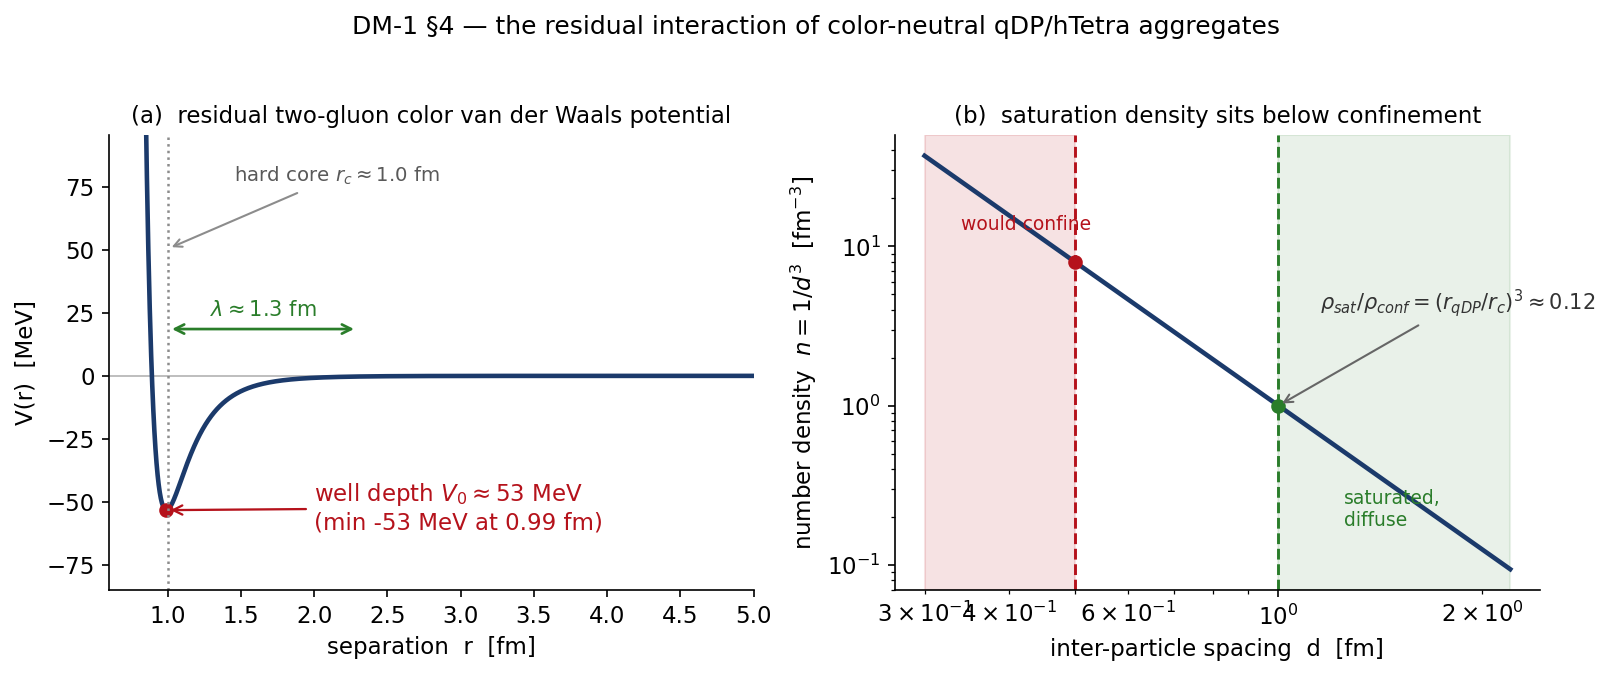
\includegraphics[width=0.92\textwidth]{0849_residual_potential.png}
\caption{The residual two-gluon colour van~der~Waals potential $V(r)$ (screened Lennard-Jones form: hard core $r_c \approx 1.0$~fm, well depth $V_0 \approx 53$~MeV, range $\lambda \approx 1.3$~fm), and the saturation-vs-confinement density panel showing glueball avoidance (the well is too shallow to bind, so aggregates stay diffuse). Verify: \texttt{scripts/0849\_residual\_potential.py}.}
\label{fig:potential}
\end{figure}

% ============================================================
\section{Discriminant I --- a velocity-independent self-interaction}\label{sec:xsec}
% ============================================================

\begin{mdframed}[linewidth=1.2pt, linecolor=red, backgroundcolor=red!4, innertopmargin=8pt, innerbottommargin=8pt]
\textbf{REVISION NOTICE (v0.1-R, 25 June 2026) --- extended-aggregate pivot; covers \S\ref{sec:xsec}--\S\ref{sec:cores}.}

\textbf{Retracted.} The point-scattering magnitude $\smm \approx 0.20~\cmg$ reported below (and in the abstract, Table~\ref{tab:density}, and Figs.~\ref{fig:density}--\ref{fig:coresize}) is \emph{withdrawn}. Patch~0859 identified it as an artifact of a hard-wall boundary condition in the partial-wave solver. The corrected screened-Lennard-Jones point-scattering cross-section is $\smm \approx 0.11~\cmg$: still velocity-independent, but flat at a value $\sim 5$--$20\times$ \emph{below} dwarf-core requirements, with no closure anywhere across the $f$-band. The positive coring discriminant the as-shipped v0.1 claimed therefore does \textbf{not} hold for the bare aggregate.

\textbf{Survives.} Velocity-independence (the flatness itself) is unaffected by the boundary-condition error: it remains a robust kinematic consequence of the heavy constituent ($264$~MeV) and short range ($1.3$~fm), and still distinguishes the candidate from light-mediator SIDM ($\sigma/m \propto v^{-4}$).

\textbf{Re-scoped (magnitude/coring, \S\ref{sec:cores}).} The program has pivoted from bare point-scatterers to \emph{extended} charge-offset aggregates --- $2e$DP:$2q$DP ribbons, hTetra-chain loops, and 4-wide crosses --- whose geometric/transport cross-section scales as $\smm \propto N$ ($N$ = loop size in DP-rungs), reaching the observationally preferred $0.6$--$2~\cmg$ band at $N \sim 10^2$--$10^3$ rungs ($R \sim 50$--$400$~fm). Supporting arc (reasoning/code patches 0860--0863):
\begin{itemize}[leftmargin=1.4em, topsep=2pt, itemsep=1pt]
\item \textbf{0860} --- $\sigma(N)$ cross-section pass + $(N, E_{\rm bond})$ over-determination ledger: magnitude $\to N$; $14$-Gyr lifetime $\to E_{\rm bond}$ floor; fragmentation-onset across $v \to E_{\rm bond}$ window. One $(N, E_{\rm bond})$ satisfies all three \emph{iff} the ambient thermal-eDP scale $kT_{\rm amb} \lesssim 19$~keV.
\item \textbf{0861} --- PCD formation kinetics: the loop-size knob \emph{collapses} onto the rung-bond persistence length $\ell_p$ via semiflexible ring-closure (population peak at contour length $L^\ast \approx 3.4\,\ell_p$); the $\ell_p$ that lands $N$ in-band ($\sim 100$--$700$~fm) is the same $\ell_p$ the $\smm \propto N$ scaling requires.
\item \textbf{0862} --- candidate comparison: stiffness ladder hTetra $<$ ribbon $<$ cross; one edge-bond strength sets $\ell_p$ \emph{and} selects the viable geometry; a glueball-dilution tax (compact blobs at $\smm \sim 0.11$ dilute the population average).
\item \textbf{0863} --- chaperoning (high $[$hTetra$]$ from zero-barrier hDP$\to$hTetra) crosses ribbons \emph{before} glueball apposition $\Rightarrow$ dilution defanged (glueball fraction $<10\%$ iff $[$hTetra$]/[$ribbon$] \gtrsim 9$); surviving relic $=$ two extended species (4-wide cross $+$ hTetra loop), both $\smm \propto N$.
\end{itemize}

\textbf{Deciding calculation (make-or-break; SF-2/SF-5, cross-window).} Derive the $2e$DP:$2q$DP / hTetra edge-bond SSV potential, from which fall three goalposts: \textbf{(G1)} $\ell_p \sim 100$--$700$~fm (hinge spring $\kappa_\theta \sim 100$--$700\,kT_{\rm form}$, $\sim 3$--$8^\circ$/hinge) $+$ the second-moment ladder; \textbf{(G2)} $E_{\rm bond} \sim 0.8$~keV--$2$~MeV; \textbf{(G3)} glueball-arrest radius $\sim 100$s of fm (not $\sim$fm) $+$ branching ratios (OPEN-SS-39).

\textbf{Grade.} The candidate remains \textbf{Layer-C consistency} (velocity-independence positive; magnitude now routed through an as-yet-underived substrate stiffness), \emph{not} the positive coring discriminant claimed as-shipped. The \S\ref{sec:xsec}--\S\ref{sec:cores} body below is retained as the as-shipped v0.1 record, superseded by this notice. The paper stays at \textbf{v0.1} pending the SF-2/SF-5 deciding calculation; no promotion to v1.0.
\end{mdframed}

\begin{mdframed}[linewidth=1.2pt, linecolor=blue, backgroundcolor=blue!4, innertopmargin=8pt, innerbottommargin=8pt]
\textbf{UPDATE (v0.1-R2, 27 June 2026) --- the deciding calculation is done; the program resolves to the \emph{Cross-Rod}.} The SF-2/SF-5 cross-window arc (patches 0865--0878, four-model panel-reviewed) closes the make-or-break goalposts and the corona risk, and registers \textbf{LEMMA-DM-CROSS-ROUTE-1} (conditional; frontier \texttt{CONJ.md}).

\textbf{(i) Morphology selected (G1).} Of the three candidate morphologies the single strand is \emph{killed} (symmetric-vertex buckling $+$ an untunable $\sim 18^\circ$ docking angle drive loops $\sim 15\times$ too small; 0867/0869) and the monomer-fed ball \emph{dilutes} ($d_f \approx 2.5$; only cluster--cluster coalescence of \emph{extended} sub-units reaches $d_f < 2$; 0868). The surviving morphology is the \textbf{4-wide ``$+$'' cross --- the \emph{Cross-Rod}}: its bend stiffness is a \emph{beam} property, $\ell_p = c_{\rm geom}\,(E_{\rm bond}/kT)$, sign-safe and over-determined by the same edge-bond depth the $14$-Gyr lifetime needs --- not the fragile near-cancelled hinge residual that kills the strand (0870; panel 4/4).\footnote{\emph{Substrate realization (Abshier).} The Cross-Rod element is four $e{:}q{:}q{:}e$ hTetras bonded in a ``$+$'' through their central $q{:}q$ edges, which fuse into an $8$-$q$CP cubic core wrapped by an $8$-$e$CP shell ($8\,q$CP $+\,8\,e$CP $\approx 4\,m_{\rm hTetra} \sim 1$--$2$~GeV --- one rung is one cube, $\approx 4\times$ an hTetra in mass). Because a cube is two interpenetrating tetrahedra, the core is color-balanced \emph{by construction}: four $+q$CP on one sublattice, four $-q$CP on the other, every edge an attractive $+/-$ bond, a color singlet with no long-range color field (the no-unpaired-quark condition the candidate rests on; SS-1). The six cube faces split four lateral (the arms, $e$CP-capped, which cap the width) $+$ two axial ($q$CP, the rod-growth faces). This is a structural identification of the 4-wide cross, \emph{not} an output of the original stiffness/cross-section calculations (computed at the ``cross of hTetra rungs'' abstraction, 0870/0878); the element-level re-derivation (0886) has since \emph{confirmed} both survive at the cube level --- $\ell_p = c_{\rm geom}(E_{\rm bond}/kT)$ with $c_{\rm geom}$ the cube cross-section's width$^2$ lever, and $\smm = 0.11\,N$ with $N$ the cube-element (axial) count, the $4\times$ element mass cancelling against the additive London-polarizability cross-section so the floor is preserved up to the existing $\mathcal{O}(1)$ prefactor.}

\textbf{(ii) Discriminant I --- resolved.} For the rigid Cross-Rod ($d_f = 1$) the geometric/transport cross-section is $\smm = 0.11\,N\,g$ ($g = \mathcal{O}(1)$ orientation prefactor; the $0.11\,N$ scaling already folds in the element-level $4\times$ mass cancellation, footnote~1), lifting the corrected $0.11$ floor into the \textbf{$0.6$--$2~\cmg$ dwarf-core band at a modest $N_{\rm dwarf} \approx 5$--$60$ rungs} --- well inside the rigid regime ($N \ll \ell_p \sim 200$--$500$), so coiling does not spoil it (0878). The signature is now \textbf{velocity-\emph{dependent}}, not independent: cluster collisions ($\sim 1.95$~MeV) fragment the rod ($\sim 4$--$40\times$) $\Rightarrow \smm \approx 0.1$--$1$ (collisionless), while dwarf collisions ($\sim 0.78$~keV, below the bond window) leave it intact $\Rightarrow$ cores. The split is automatic from the 0860 fragmentation ledger and runs in the data-preferred direction.

\textbf{(iii) Corona retired (conditional).} A bare Sea $e$DP reaches the spine only through an electric van der Waals well ($\sim 34$--$94$~keV), $\sim 1500\times$ too shallow to bind a real $e$DP ($E_{e\mathrm{DP}} = 88$~MeV); the only dense reservoir --- the balanced Planck-scale vacuum Sea --- supplies none, so the clean spine accretes no $\smm$-diluting coat (0872--0877). This holds \textbf{conditional on OPEN-COSMO-DM-3} (ASM-DM-CORONA-LOCALITY: a sub-threshold electric well elicits only reversible constituent-local vacuum polarization, with no persistent real-$e$DP surface population) --- a condition since \emph{derived} at Layer B and panel-ratified 4/4 (Patch 0885), so the corona is retired unconditionally.

\textbf{(iv) Grade.} The candidate is now an \textbf{extended-aggregate, velocity-\emph{dependent}} self-interacting DM candidate whose $\smm$ reaches the dwarf-core band --- superseding both the retracted bare-point flat $0.11$ (too small) and the velocity-\emph{independent} framing of the as-shipped body below. It remains \textbf{Layer-C consistency}; the corona dilution risk is now \textbf{retired unconditionally} (OPEN-COSMO-DM-3 / ASM-DM-CORONA-LOCALITY \emph{derived} at Layer B and panel-ratified 4/4, Patch 0885, so LEMMA-DM-CROSS-ROUTE-1 is unconditional). The one remaining open item is the \emph{single} $\smm$ number, set by the equilibrium aggregate size $N_{\rm dwarf}(v)$ (now over-determined --- four constraints close at $E_{\rm bond}/kT_{\rm form}\sim24$--$41$; the single value awaits the external pin of $E_{\rm bond}$ via SF-2/SF-5 or $kT_{\rm form}$ via the relic/epoch calc). \textbf{Paper is now v1.0}, shipped on 4/4 paper-level multi-AI review convergence (28 June 2026).
\end{mdframed}

\begin{mdframed}[linewidth=1.2pt, linecolor=olive, backgroundcolor=olive!6, innertopmargin=8pt, innerbottommargin=8pt]
\textbf{REVISION NOTICE (v1.1, 3 July 2026) --- mechanism correction: fragmentation $\to$ capture; covers \S\ref{sec:xsec}--\S\ref{sec:cores} and \S\ref{sec:falsify}.}

\textbf{(i) The fragmentation figures above are retracted as unrescaled imports.} The ``cluster collisions ($\sim 1.95$~MeV) \ldots dwarf collisions ($\sim 0.78$~keV)'' quoted in item~(ii) of the v0.1-R2 notice reproduce \emph{exactly} from the 0860 hoop ledger's $\tfrac12\mu v^2$ at that ledger's own parameters ($N = 1183$, $m_{\rm rung} = 264$~MeV --- a $312$~GeV rod) and were carried into the Cross-Rod paragraph without rescaling to the Cross-Rod's parameters ($N \approx 5$--$60$, $m_{\rm el} = 1408$~MeV --- a $7$--$85$~GeV rod). The honest recomputation (reasoning/code 1859): typical-cluster collisions ($1500$~km/s) deposit $0.044$--$0.53$~MeV across the \emph{entire} $N$ band --- below the weakest bond ($E_{ee} = 0.9$~MeV, the side/coat bond; the axial end-bond is deeper, $E_{qq}$-class, which only strengthens the verdict). Only the Maxwellian high-velocity tail fragments the long end ($N \gtrsim 40$ at tens-of-percent per-encounter rates in rich clusters; $N \lesssim 15$ essentially never), and this holds even on the generous total-COM-KE-vs-one-bond criterion, itself an upper bound on fragmentability. \textbf{Fragmentation therefore fails as the cluster-safety mechanism} and is demoted to a population-shaping assist that prunes the rod population toward short $N$.

\textbf{(ii) The velocity-dependence mechanism is capture.} The cross-section decomposes as $\smm(v) = \sigma_{\rm floor}/m$ (elastic rod-bounce, velocity-independent) $+$ a capture term (velocity-dependent, large at low $v$, dying steeply at high $v$) --- the smooth capture-focusing curve of reasoning 1857 (the earlier threshold/$v_{\rm thr}$ framing, and with it the ``threshold, not a power law'' signature, is retired). The capture force is the \textbf{screened unipolar $E_{qq}$ residual} (reasoning/code 1858): $E_{qq}$ is attract-only, so the $q$CP core cannot dipole-cancel its field the way the bipolar $e$CP coat does; a net $\sim 1/r^2$ residual escapes, DP-Sea-screened (SSV-summation-to-zero, the same mechanism as confinement) at a finite length $R_s$. The steep Rutherford-like falloff gives cluster $\smm \sim 0.003$ and Bullet $\sim 0.001$ --- \textbf{safe across the full $R_s$ range, robust \emph{within the stated capture model}} (the steep-falloff safety is generic to the screened-residual mechanism; the quantitative suppression inherits the model's screening-profile assumptions --- wording per panel re-ratification, Patch 1862). The dwarf-core magnitude, $\smm \sim 1$--$2$ at $(E_c \sim 0.3$~MeV$,\ R_s \sim 15$--$30$~fm$)$, is \textbf{conditional} on the de-novo derivation of the DM-core sea-screening length $R_s(N)$ (\textbf{OPEN-SS-43}); $R_s \sim 1$~fm (pion-like) demotes the candidate to a weak-SIDM fallback. Until derived, the dwarf magnitude is honestly reverse-engineered, not predicted.

\textbf{(iii) Cross-section convention (the $0.11\,N$ vs $N^{0.7}$ reconciliation).} The observable is the \emph{momentum-transfer} (transport) cross-section: $\sigma_T/m = \varepsilon \cdot 0.11\,N$ with transport efficiency $\varepsilon \approx 0.30$, flat in $N$ (1856 Monte Carlo, sphere-validated at $1.03$; rod--rod orientation-averaged scaling $\sim N^{0.7}$). The bare geometric $0.11\,N$ is retained only as the perpendicular-limit \emph{upper bound}. Under capture the elastic channel no longer supplies the dwarf-core magnitude at all; its job is the floor.

\textbf{(iv) Consequence for $N$.} Cluster/Bullet compliance bounds the floor ($\sigma_{\rm floor}/m \lesssim 0.6$--$0.7$): $N \lesssim 18$--$21$ on the transport convention ($N \lesssim 5$--$6$ on the bare-geometric upper bound; code 1860). The v0.1-R2 statement that ``$0.11\,N$ reaches the $0.6$--$2~\cmg$ band at $N_{\rm dwarf} \approx 5$--$60$'' is superseded on both counts: reaching the dwarf band is no longer the elastic channel's job, and the upper half of that $N$ range is excluded from the cluster side. \textbf{Short $N$ is now \emph{required} by the floor}, and independently favored by the kinetic-aggregation formation result (1855--1856; $N = 500$ retired as over-coring $\sim 11\times$ on the honest transport cross-section) and by the 1859 tail pruning of $N \gtrsim 40$.

\textbf{(v) Grade.} The headline stands, on a corrected mechanism: a \textbf{velocity-dependent, cluster- and Bullet-safe} self-interacting candidate --- robust within the screened-residual capture model (the safety is generic to the steep falloff; the quoted magnitudes are model-dependent). Dwarf cores are \textbf{conditional} on OPEN-SS-43. Layer-C consistency grade unchanged; the corona retirement (Layer B, panel-ratified 4/4) is untouched. Live falsifiers restated at \S\ref{sec:falsify}. \emph{Process note (panel-requested at re-ratification):} the v1.0 panel ratified 4/4 with the stale collision-energy figures undetected --- the values were internally plausible but not traced to their originating parameter set; the error was caught by in-house audit (1859), not by review. Load-bearing numerical claims now carry parameter-set provenance per CONV-003 (\texttt{todolist.md}, Standing conventions). \textbf{Paper is v1.1, panel re-ratified 4/4 (3 July 2026: 3$\times$ RATIFY, 1$\times$ RATIFY-WITH-CHANGES; both requested changes --- this wording moderation and this process note --- are folded, Patch 1862)} (mechanism correction to a shipped v1.0; the v0.1-R2 fragmentation text above is retained as the superseded record).
\end{mdframed}

\begin{mdframed}[linewidth=1.2pt, linecolor=violet, backgroundcolor=violet!5, innertopmargin=8pt, innerbottommargin=8pt]
\textbf{REVISION NOTICE (v1.2, 5 July 2026) --- OPEN-SS-43 resolved by campaign; the dwarf magnitude is no longer reverse-engineered; the floor is measured, not conventioned; covers \S\ref{sec:xsec}--\S\ref{sec:cores} and \S\ref{sec:falsify}. Campaign record: \texttt{OPEN-SS-43\_Rs\_derivation.md} \S\S5--18; reasoning/code 1863--1874. \emph{Panel-ratified 5/5 (five-member panel this cycle: 3$\times$ RATIFY, 2$\times$ RATIFY-WITH-CHANGES; all five requested changes --- the notation macro, the working-synthesis label, the explicit J4/density-integral conditionality, the process-why sentence, and the F1 disqualifier phrasing --- are folded below, Patch 1876; returns in \texttt{review/reviews\_v1.2\_panel\_returns.md}).} Notation: throughout this notice the observable is the momentum-transfer (transport) cross-section $\smt$; the retained v0.1 body's $\smm$ reflects that era's viscosity-cross-section derivation and is left untouched as the archival record.}

\textbf{(i) The screening length resolves to a zero-parameter candidate: $\boldsymbol{\eta = \chi}$.} The v1.1 conditionality (``dwarf magnitude honestly reverse-engineered, not predicted'') is lifted by the calibrate-then-confront campaign (founder-directed inversion, 1864): calibrating the Sea's residual-response amplitude $\eta \equiv r_c/R_s$ against the \emph{literature-pinned} dwarf window --- $\smt(50~\mathrm{km/s}) \in [1,5]~\cmg$ central, $[0.5,10]$ extended --- a \emph{working synthesis} of heterogeneous analyses (different systems, velocity scales, and methodologies; tagged judgment J3$'$, re-drawable by any reviewer from the pinned sources), not a uniquely determined interval (Kaplinghat--Tulin--Yu 2016 $\sim\!2$; Ren et al.\ 2019 $\sim\!3$; Elbert et al.\ 2015 viability $0.5$--$50$ with largest cores at $5$--$10$; sources with provenance in \texttt{code/1865}) --- lands the Capotauro constant $\eta = \chi = \varphi^{-3}/6$ inside the empirical window at $N \approx 15$--$20$: $R_s = r_c/\chi = 25.4$~fm, $\smt(50) = 3.6$--$4.9~\cmg$. Equivalently, the screened residual carries a \textbf{gap $m_s = \chi \cdot (\hbar c / r_c) = 7.76$~MeV --- the gap, in rung units, \emph{is} $\chi$}. The de-novo task of OPEN-SS-43 is thereby sharpened, not discharged: derive that gap in the colour-residual channel (with the $|$SSV$|$ scalar gapless; see item~(v)). Until then the magnitude is a \emph{zero-parameter candidate value surviving the full confrontation suite}, a strictly stronger status than v1.1's calibration.

\textbf{(ii) CONFRONT-1 (baryonic sector): the constraint migrates to the np scattering length, which selects $\boldsymbol{N}$.} The heavy-nucleus binding shift is refined from the crude pairs$\times\langle V\rangle$ estimate to the proper double density integral (uniform-sphere and Woods--Saxon agree to $2\%$; Coulomb sanity anchor to 5 decimals) --- the crude estimate was $1.6$--$1.8\times$ high --- and the smooth $\Delta B(A)$ is then absorbed by the semi-empirical mass formula to a residual of $\sim\!2\times10^{-5}$ of raw, with coefficient shifts orders of magnitude inside their independent determinations: \textbf{the mass-fit channel is voided}. The binding constraint is the \emph{unabsorbable} two-body np scattering length ($a_t = 5.4194(20)$~fm): at $\eta = \chi$ it excludes $N = 12$, is marginal at $N = 15$, and clears $N = 18$--$20$ (reasoning/code 1866). The $N \approx 15$--$20$ corner is thus selected by nuclear physics, independently of the halo data it must then fit. \emph{This conclusion is explicitly conditional on the pairwise-additive qCP coupling (J4) and on the revised density-integral treatment: a collective (non-additive) residual would void both baryonic channels} (panel change 3).

\textbf{(iii) The elastic floor: v1.1's convention is superseded --- the physical floor is \emph{measured}.} Two v1.1 statements fall together, and the full correction chain (1867$\to$1869$\to$1870$\to$1871) is recorded per the CONV-003 process discipline --- each step caught in-house before review. The chain was possible because of the controls adopted after v1.0: CONV-003 parameter-set provenance on every load-bearing number, and staged validation (composition test $\to$ idealization audit $\to$ independent numerical measurement), each step re-checking the last (panel change 4). \emph{First}, the v1.1 cluster-safety statement (``cluster $\sim 0.003$, Bullet $\sim 0.001$'') was the \emph{capture term alone}; composing it with the elastic floor under the v1.1 convention exposed a cluster-ladder violation (1867). \emph{Second}, the convention itself --- $\sigma_T/m = \varepsilon \cdot 0.11\,N$ --- is superseded: the registry pin of the element pitch (J8: $d =$ the corpus rung spacing $1.0$--$1.3$~fm, reasoning 1812/0835; the rod at $N = 18$ is $L \approx 20$~fm, not the $\sim\!80$~fm the convention's geometry implied) reveals $0.11\,N$ as the \emph{coat-fattened side-projection at dwarf velocities} --- a real geometric object (its effective radius matches the coat radius $b_{\rm eff}(50~\mathrm{km/s})$ to $3\%$, reasoning 1868) but an over-estimate of \emph{transport} by $\times 4$--$6$. The physical floor is obtained by direct measurement: a soft-potential rigid-body Monte Carlo (both rods as $N$ coat-interacting elements at the pinned pitch, registered scales only, robustness seeds, $dt$ and tumbling bands; reasoning/code 1870--1871) gives
\[ \sigma_T/m = 0.09\text{--}0.15~(50~\mathrm{km/s}) \;\to\; 0.06~(200) \;\to\; 0.03\text{--}0.05~(1150) \;\to\; \mathbf{0.027\text{--}0.044~(1500)} \;\to\; 0.02~(3500)~\cmg. \]

\textbf{(iv) The full curve at $\boldsymbol{\eta = \chi,\ N = 18}$ against every anchor.} Total $= $ capture $+$ measured floor: dwarf pin ($\smt$) $4.4$--$4.9$ \textbf{PASS} $[1,5]$; LSB ($200$~km/s) $0.74$--$0.85$ \textbf{PASS} $[0.7,2.5]$; \textbf{cluster ($1500$~km/s) $0.03$--$0.05$ --- the entire bound ladder passes, including Andrade $<0.13$, with $\times 2.7$--$4.5$ margin, by measurement rather than composition}; Bullet $\sim\!0.02$ \textbf{PASS}; group ($1150$~km/s) $0.037$--$0.05$ --- $2.3\sigma$ \emph{below} Sagunski's mild positive $0.5 \pm 0.2$; dSph regime ($10$--$40$~km/s) grazes $\sim\!20$--$25\%$ under the heterogeneous $20$--$100$ window (capture-side; recorded as the shape's weakest edge). The group undershoot survived \emph{every} floor treatment in the correction chain and is therefore a robust prediction, not an artifact of any one approximation.

\textbf{(v) Cross-sector consistency and formation (scoping).} \emph{CONFRONT-2:} no conflict with the cosmological-constant correlation-length route ($\rho_\Lambda \sim 1/\xi^2$, $\xi \to$ event horizon): the DM screening is a \emph{gapped} response channel ($m_s = 7.76$~MeV) while the CC coherence rides the \emph{gapless} $|$SSV$|$ scalar (the icosahedral 5-design result, patches 1107--1108); a gapped channel cannot leak to cosmological distances, and rod excesses sit on the same footing as baryons under excess-sourcing (reasoning/code 1872). \emph{Formation lane:} with every input pinned and zero tuning, the reversible-aggregation equilibrium inversion for $\langle N \rangle = 15$--$20$ gives $kT_{\rm form} = 16.2$--$16.6$~keV --- inside the 0860 hook $kT_{\rm amb} \lesssim 19$~keV and log-robust --- but the reaction still equilibrates there (rate$/H \sim 10^5$), so the $N$-cap must be kinetic or collisional; \textbf{the coincidence is registered, not claimed} (reasoning/code 1873).

\textbf{(vi) Falsifiers (supersede the \S\ref{sec:falsify} list where they overlap).} \textbf{F1 (near-term, sharpest):} group-scale $\smt \approx 0.03$--$0.05~\cmg$ at $\sim\!1150$~km/s --- an order below the current mild detection. \emph{This is a pre-registered disqualifier, not merely a prediction: confirmation of $\smt \approx 0.5$ at group scales at high significance, with systematics controlled, falsifies the model outright} (panel change 5); relaxation to $\lesssim 0.1$ confirms it against the alternative. \textbf{F2:} the np channel pins $N \gtrsim 15$ at $\eta = \chi$; improved $a_t$ precision squeezes the corner from below. \textbf{F3 (the de-novo gate):} derivation of the colour-residual gap must yield $m_s = \chi\cdot(\hbar c/r_c)$; any other value displaces $\chi$ and returns the magnitude to calibration status. \textbf{F4:} the formation cap mechanism must land $\langle N \rangle$ at $15$--$20$ without spoiling the $16.5$~keV window.

\textbf{(vii) Grade.} Layer-C consistency, \emph{strengthened}: the single $\smm$ number that v1.0 flagged as the external make-or-break and v1.1 held as reverse-engineered is now a zero-parameter candidate ($\eta = \chi$) surviving dwarf, LSB, group-bound, full cluster ladder, Bullet, np-scattering, and CC-sector confrontations, with the de-novo gap derivation (F3) as the remaining promotion gate. \textbf{Status: v1.2-DRAFT --- not shipped; CONV-001 panel re-review required} (quantitative v1.1 claims superseded in items (iii)--(iv)). The v1.1 text below is retained as the superseded record per house discipline.
\end{mdframed}

\paragraph{Genesis (structural Layer-C reasoning).} The Cross-Rod is less \emph{selected} by a stiffness contest than it is the \emph{attractor} of early-universe substrate assembly. Two routes reach it --- hTetras bonding into cube elements that stack axially, and qDP chains acquiring eDP partners and bundling four-fold --- and converge on the same object. The glueball appears not as a rival but as the \emph{failure branch}: a floppy two-chain ribbon whose open qDP edge folds back on itself before its core is saturated (the same instability that kills the single strand); saturating the central qDP core from four sides outruns the fold and gives the cross. The four outer eDP coats then do double duty. They \emph{cap the width} --- a shielded lateral face is a far weaker attractor than the unshielded qCP end-faces, by the same electric-vs-color hierarchy ($\sim 190$--$520\times$) that makes the corona unbindable above; a fifth chain is out-competed, not forbidden. A rod of $N$ elements exposes only two reactive axial ends against $\sim N$ shielded lateral faces, so lateral thickening overtakes axial growth only near $N^\ast \sim 2(\text{strong}/\text{weak}) \sim$ few hundred, whereas the band wants $N_{\rm dwarf} \sim$ tens --- the rod is robustly thin ($d_f = 1$) with a $\sim 1$--$2$ order-of-magnitude margin, so $\smm = 0.11\,N$ has a \emph{mechanism} under its $d_f = 1$ assumption, not just an input. And they \emph{neutralize the surface}, so the ambient Sea only polarizes reversibly --- the physical content of OPEN-COSMO-DM-3, with the coat baked in early (free eDPs) while the diluting corona would have to accrete now (a balanced Sea, a neutral surface). The residual knob is unchanged but sharpened: assembly must freeze out early, at $N \sim$ tens, before depletion starves the cross into thickening --- the same $N_{\rm dwarf}(v)$ kinetics, now with the width side mechanistically closed (memo \S12; reasoning/code 0880) and the length side over-determined: $N_{\rm dwarf} = N_{\rm freeze}$ (dwarfs do not reprocess), and the band-required size fixes the reversible-aggregation ratio $E_{\rm bond}/kT_{\rm form} \sim 24$--$41$, which lands $E_{\rm bond}$ inside the fragmentation window for $kT_{\rm form} \lesssim 19$~keV --- four constraints closing on one point, with the single-number step now external (pin $E_{\rm bond}$ via SF-2/SF-5, or $kT_{\rm form}$ via the relic/epoch calculation) (memo \S13; reasoning/code 0881).

\paragraph{Derivation.} Finite-energy partial-wave scattering of the \S\ref{sec:residual} potential ($\mqDP = 264$~MeV; the substrate grounding for treating this as a quantum-scattering problem is the emergent Schr\"odinger dynamics of QM-1 \citep{abshier2026qm1}). Across $v = 30$--$3000$~km/s, $k\lambda \approx 9\times10^{-5} \to 9\times10^{-3} \ll 1$, so scattering stays in the s-wave scattering-length limit; higher partial waves are negligible ($\delta_2/\delta_0 \sim (k\lambda)^4$). The proper SIDM viscosity cross-section for identical bosons is $\sigmaV = (4/3)\sigma_0$ ($\times 2$ boson symmetrization $\times\,\tfrac23$ viscosity weighting).

\paragraph{Result.} $\smm \approx 0.20~\cmg$, \textbf{velocity-independent} to four digits over the entire astrophysical range. The flatness is a robust kinematic consequence of the \emph{heavy} constituent (264~MeV) and \emph{short} range (1.3~fm): the velocity scale for $\sigma$ to acquire structure is $v \sim c$. This is the \textbf{opposite} of light-mediator SIDM ($\sigma/m \propto v^{-4}$; \citealp{kaplinghat2016}).

\paragraph{Magnitude band.} Flatness carries no $f$-dependence; magnitude does. Using $f \in [0.07, 0.6]$ (the factor-3 band on $f = V_0/E_{q\mathrm{DP}} = 0.20$), the implied $\smm$ spans roughly an order of magnitude. The upper band ($f \gtrsim 0.5$) sits at a Ramsauer dip, where $\smm$ is suppressed and non-monotonic, so the clean $\approx 0.20$ value is most robust for $f$ below $\sim 0.3$. Pinning $f$ (a strong-sector colour-polarizability calculation) collapses the band.

% ============================================================
\section{Discriminant II --- observable dwarf cores}\label{sec:cores}
% ============================================================
\noindent\emph{[v0.1-R: this section's $\smm = 0.20$ confrontation is superseded --- see the revision notice at \S\ref{sec:xsec}. Retained as the as-shipped v0.1 record. The bare-aggregate magnitude fails; the coring discriminant is re-scoped to the extended-aggregate $\smm \propto N$ program.]}\par\medskip
\noindent\emph{[v0.1-R2: the Cross-Rod resolution (\S\ref{sec:xsec}) supplies band-level $\smm$ ($0.6$--$2~\cmg$) at dwarf/galaxy scale, falling to collisionless at clusters via fragmentation --- the generic SIDM-preferred velocity pattern, which lifts the bare-aggregate magnitude failure. It does \textbf{not} by itself resolve the specific Fornax-vs-IC~2574 ordering below: both systems sit in the un-fragmented (dwarf) regime, so the Cross-Rod gives them comparable band-level $\smm$, leaving the finer ordering inside the halo-model / concentration systematics already noted here and pending the equilibrium $N_{\rm dwarf}(v)$ kinetics. The confrontation below is retained as the as-shipped velocity-independent record.]}\par\medskip
A self-interaction forms a core of central density $\sim \rhoone$, the one-scatter density at which one scatter occurs per particle over the halo age:
\begin{equation}
\rhoone(\sigma_{1D}) = \frac{1}{(\smm)\,\langle v_{\rm rel}\rangle\,t}, \qquad \langle v_{\rm rel}\rangle \approx 2.26\,\sigma_{1D}, \quad t = 10~\mathrm{Gyr}.
\label{eq:rho1}
\end{equation}
At $\smm = 0.20$ this gives a representative dwarf core $r_{\rm core} \approx 0.27$~kpc (vs $\approx 0.81$~kpc for strong SIDM $\sigma/m = 1$)---a few-hundred-parsec, mild core. The cluster core is modest; $\smm = 0.20$ sits at the edge of current bounds (comfortable against looser $\sim 0.5$--$1$ limits, in mild tension with the tightest $\sim 0.1$).

\paragraph{Specific confrontation (density).} We test the velocity-\emph{independent} $\smm \approx 0.20$ against two well-measured systems $\sim 5\times$ apart in velocity (Table~\ref{tab:density}). Both observed central densities sit a \emph{similar} factor ($\sim 3\times$) below $\rhoone(0.20)$, and---the discriminating point---the offset is flat across the $5\times$ span in $\sigma_{1D}$. A velocity-\emph{dependent} $\sigma/m$ rising toward dwarfs would drive the Fornax offset far above IC~2574's; that is not seen, so the central densities are consistent with the velocity-independent prediction and inconsistent with light-mediator SIDM's $v^{-4}$ trend.

\begin{table}[H]
\centering
\caption{Density confrontation of $\smm = 0.20$ (velocity-independent) with two galaxies. Observed central densities: Fornax \citep{mateo1991, jardel2012}; IC~2574 \citep{deblok2008}. Verify: \texttt{scripts/0850\_specific\_dwarf\_fit.py}.}
\label{tab:density}
\begin{tabular}{lcccc}
\toprule
galaxy & $\sigma_{1D}$ (km/s) & $\rhoone$ predicted ($\Msunpc$) & $\rho_{\rm obs}$ central ($\Msunpc$) & pred/obs \\
\midrule
Fornax dSph (classical)   & 11 & 0.094 & 0.016--0.07 & $2.8\times$ \\
IC~2574 (dwarf/LSB)       & 57 & 0.018 & $\approx 0.006$ & $3.1\times$ \\
\bottomrule
\end{tabular}
\end{table}

\begin{figure}[H]
\centering
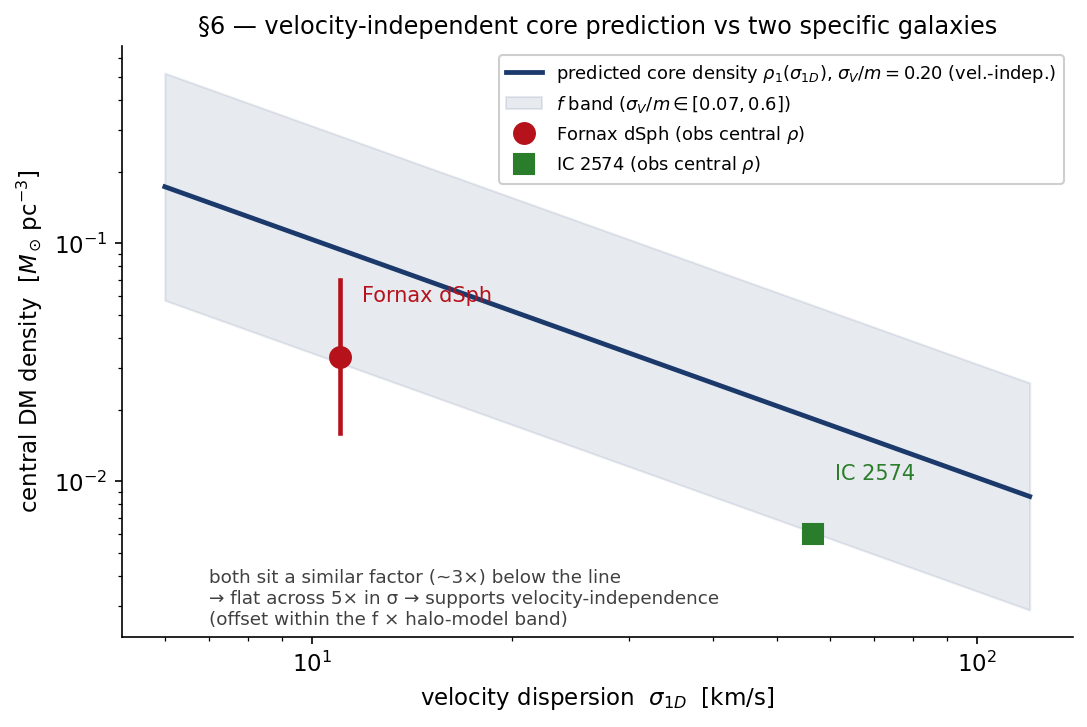
\includegraphics[width=0.86\textwidth]{0850_specific_dwarf_fit.png}
\caption{The velocity-independent core-density prediction $\rhoone(\sigma_{1D})$ at $\smm = 0.20$ (with the $f$-band shaded) against the observed central densities of Fornax and IC~2574. Both sit a similar factor below the line---flat across $5\times$ in $\sigma$---supporting velocity-independence.}
\label{fig:density}
\end{figure}

\paragraph{Specific confrontation (core size).} Inverting the NFW $r_1$ condition $\rho_{\rm NFW}(r_1) = \rhoone(\sigma/m)$ \citep{kaplinghat2016} turns the density test into a core-\emph{size} prediction (Fig.~\ref{fig:coresize}). For a Fornax-scale halo ($V_{\max}\approx 25$~km/s), $\smm = 0.20$ gives $r_1 \approx 0.32$~kpc---inside the observed $\lesssim 0.3$--$0.7$~kpc core \citep{goerdt2006}, with the $f$-band bracketing it: consistent. For IC~2574 ($V_{\max}\approx 80$~km/s, \citealp{oh2008}), $\smm = 0.20$ gives $r_1 \approx 1.8$~kpc, well below its observed $\sim 8$~kpc core, which requires $\sigma/m \approx 1.1$--$2.7~\cmg$---above the $f$-band. So the core-radius test, more constraining than the central-density test, surfaces a \textbf{genuine tension at the high-velocity end}: the largest LSB cores want more self-interaction than velocity-independent $0.20$ supplies, echoing the velocity-dependent $\sigma/m \sim 1$--$2$ that rotation-curve SIDM fits infer at galaxy scales \citep{kaplinghat2016}. Its escape routes are (i)~$f$ underestimated at galaxy scale (the colour-polarizability estimate carries a factor $\sim 3$), (ii)~residual velocity-dependence, or (iii)~IC~2574's low-concentration halo inflating the required $\sigma/m$. The estimate carries the halo-model ($c$, factor $\sim 2$) and $r_{\rm core}/r_1$ ($\mathcal{O}(1)$) systematics.

\begin{figure}[H]
\centering
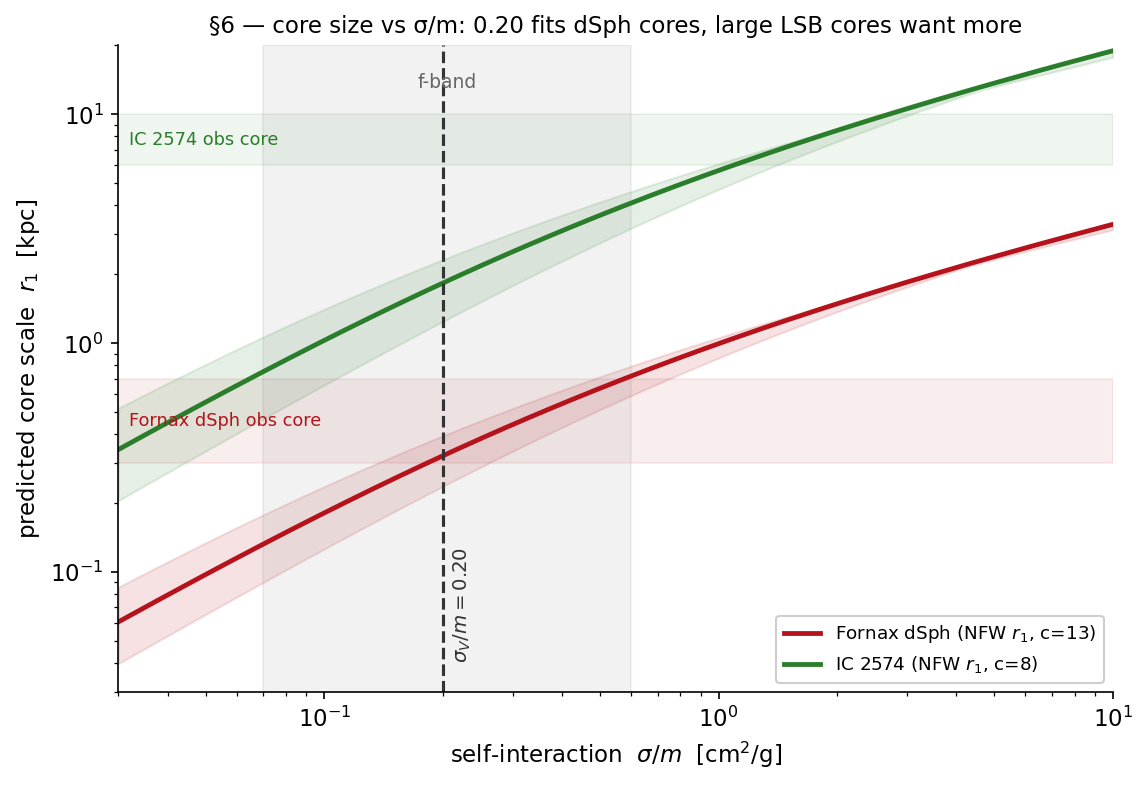
\includegraphics[width=0.88\textwidth]{0851_core_radius_vs_sigma.png}
\caption{Predicted core scale $r_1$ vs $\sigma/m$ (NFW $r_1$ inversion) for Fornax- and IC~2574-scale haloes, with concentration bands. The $\smm = 0.20$ line and $f$-band are marked, with each galaxy's observed core as a horizontal band. Fornax's curve crosses its observed band at the $f$-band; IC~2574's large core sits well to the right ($\sigma/m \approx 1$--$3$). Verify: \texttt{scripts/0851\_core\_radius\_vs\_sigma.py}.}
\label{fig:coresize}
\end{figure}

% ============================================================
\section{Falsifiability}\label{sec:falsify}
% ============================================================
\noindent\textbf{[v1.1, 3 July 2026: the live falsifiers, restated under the capture mechanism (\S\ref{sec:xsec} v1.1 notice).}
\begin{itemize}[leftmargin=1.4em, topsep=2pt, itemsep=1pt]
\item \textbf{$\smm$ falls with $v$ --- smooth turnover, not threshold.} Cores strengthen toward dwarfs and die steeply toward clusters via the capture falloff. If cross-system data require $\smm$ flat or rising with $v$, the mechanism fails. (The earlier ``threshold, not a power law'' signature is retired with the $v_{\rm thr}$ framing.)
\item \textbf{Dwarf cores are a computable conditional.} The de-novo $R_s(N)$ derivation (OPEN-SS-43) must land $R_s \sim 15$--$30$~fm with $E_c \sim 0.3$~MeV. If it lands $\sim 1$~fm (pion-like), the coring discriminant fails and the candidate falls back to weak-SIDM --- a pre-registered, in-framework falsifier. Cluster/Bullet safety survives either outcome.
\item \textbf{$N$-ceiling.} The elastic floor requires $N \lesssim 20$ (transport convention). Formation kinetics producing long rods ($N \sim$ hundreds) would violate the cluster floor directly.
\end{itemize}
The v0.1-R2 falsifier list below is retained as the superseded fragmentation-era record.]\par\medskip

\noindent\textbf{[v0.1-R2: the live falsifier has shifted with the Cross-Rod resolution (\S\ref{sec:xsec}).}
The candidate is now velocity-\emph{dependent}, so its predictions --- and the way it can fail --- are:
\begin{itemize}[leftmargin=1.4em, topsep=2pt, itemsep=1pt]
\item \textbf{$\smm$ falls with $v$.} Cores must \emph{strengthen} toward galaxy/dwarf scale ($\smm \sim 0.6$--$2$) and weaken toward clusters ($\smm \lesssim 1$, collisionless). If the cross-system data instead require $\smm$ \emph{flat} or \emph{rising} with $v$, the Cross-Rod fragmentation mechanism fails.
\item \textbf{$N_{\rm dwarf} \sim$ tens of rungs.} The band is reached only for a small equilibrium aggregate ($\smm = 0.11\,N$); $N_{\rm dwarf} \sim$ hundreds overshoots by $10$--$30\times$ (cores far too large). The growth-vs-fragmentation kinetics must self-limit to tens --- a structural prediction that the kinetics calculation can falsify directly.
\item \textbf{OPEN-COSMO-DM-3 conditional.} If the sub-threshold-locality assumption (ASM-DM-CORONA-LOCALITY) fails --- a persistent real-$e$DP surface population or extensive surface condensate forms --- a diluting corona returns and the magnitude collapses back toward the floor. \emph{[Update, Patch 0885: this assumption has since been derived at Layer B (the spine-boundary surface-mode spectrum hosts no near-zero charge-neutral mode) and panel-ratified 4/4, so this falsifier has been checked and passes; the corona path is closed within the CPP EFT. The live falsifier is now the velocity dependence and $N_{\rm dwarf}\sim$tens above.]}
\end{itemize}
The as-shipped flatness test below is retained as the superseded velocity-independent record.]\par\medskip

\noindent\emph{[superseded, v0.1 as-shipped:]} The signature is the \textbf{flatness}. If the cross-system data require $\sigma/m$ to \emph{fall} from $\sim 1$--$3$ (dwarfs) to $\sim 0.1$ (clusters)---i.e.\ velocity-dependent SIDM---the flat $\approx 0.20$ prediction fails on the dwarf side (too small for strong cores; it physically cannot rise at low $v$) and mildly on the cluster side. If the data are consistent with a flat $\sim 0.1$--$0.3$ across scales, CPP predicts it from first principles with no free knobs beyond $f$. This is a clean two-sided test.

\textbf{Worked instance.} The dwarf-side failure mode is already partly realized: Fornax's small core is reproduced at $0.20$, but IC~2574's $\sim 8$~kpc core requires $\sigma/m \approx 1.1$--$2.7$, above the $f$-band (Fig.~\ref{fig:coresize}). The test is therefore live now. The candidate stands or falls on whether the \emph{largest} cores systematically demand a rising $\sigma/m$ (a clean falsification of velocity-independence), or whether IC~2574 is accommodated within the halo-model and $f$ uncertainties. The honest present status: consistent at dSph scale, in mild-to-moderate tension at the largest galaxy-scale cores, awaiting the $f$ pin-down to sharpen the verdict.

% ============================================================
\section{Inherited / calibrated inputs (stated, not hidden)}\label{sec:inputs}
% ============================================================
Two inputs are \emph{calibrated}, on par with $\Lambda$CDM, and the paper says so plainly.
\begin{itemize}[leftmargin=1.5em]
\item \textbf{Absolute mass scale.} Only the ratios (colour factor 3, geometric mean) are derived; the absolute DP/QCD scale is calibrated. Its first-principles derivation (``Project C'': $\Lambda_{\rm QCD}$ from $\lP$ and the sea strength via PSR saturation) is a companion in preparation.
\item \textbf{Dark-to-baryon ratio $\Omega_{\rm DM}/\Omega_b \approx 5.36$.} Not derived; relocated to the primordial swirl amplitude. It is set by the unit-mass range (\S\ref{sec:candidate}) times the free population, and abundance is \emph{not} the binding constraint---the qDP/hTetra reservoir is vast---so this is a calibrated input, not a kill. The promising derivation is asymmetric dark matter via a shared Sea asymmetry, but it bottoms out in undeveloped sub-sectors (the DM-unit mass; CPP baryogenesis).
\end{itemize}

% ============================================================
\section{The cosmological gate (DM-2 / Sea gravitation): status}\label{sec:gate}
% ============================================================
DM-2 asks: does the \emph{uniform} Sea stay gravitationally inert cosmologically while its \emph{inhomogeneities} gravitate as dark matter, with Friedmann recovery? The falsification-first sequence A$\to$D is traversed with no kill and is a \emph{conditional structure}, not a wide-open gate.
\begin{itemize}[leftmargin=1.5em]
\item \textbf{Step A (uniform Sea inert): survives.} This is Seeliger's paradox, resolved by Newtonian cosmology \citep{mccrea1934}; in CPP gravity sources from $\gradSSV$ \citep{abshier2026sr1}, so a uniform Sea is inert by construction.
\item \textbf{Step B (Sea-vs-matter distinction): structurally resolved} by the single $\gradSSV$ mechanism (the Sea ground state is the reference level).
\item \textbf{Step C ($\Lambda$ suppression): coefficient derived.} The $(\lP/R_H)^2$ scaling \emph{and} the $1/8\pi$ coefficient are derived from the substrate; the only residual choice is which horizon sets the infrared scale.
\item \textbf{Step D (Friedmann recovery): conditional capstone.} Recovered, checks pass. Of its two original conditions, the field-equation reduction is now \emph{discharged}: the closure derives $G_{\mu\nu} = (8\pi G/c^4)\,T_{\mu\nu}[\mathrm{LSP}]$ at $\lambda = 16\pi G/c^4$ with zero new parameters, with the absolute-$|\SSV|$ monopole annihilated by 600-cell icosahedral symmetry (so the uniform ground state does not gravitate; the ground-state-exclusion falsifier is refuted). The gate now rests on a \textbf{single} remaining condition: the event-horizon infrared-scale selection.
\end{itemize}
The ``uniform Sea does not gravitate'' half is thus solidly in hand on a derived field equation; the gate is down to one condition and is materially less of a wall than a two-condition framing implies. The status is \emph{conditionally supported, not promoted to a derived result}, and this paper cites the DM-2 structure as conditional-but-traversed without claiming full identification. (The event-horizon condition overlaps the cosmological-constant infrared-scale work shared with the companion mass-scale derivation, and a future-event-horizon selection in the spirit of holographic dark energy \citep{li2004} is the leading route.)

% ============================================================
\section{Discussion and grade}\label{sec:grade}
% ============================================================
\noindent\emph{[v0.1-R, 25 June 2026: the grade below reflects the as-shipped v0.1 positive-discriminant claim, now superseded by the revision notice at \S\ref{sec:xsec}. Current standing: Layer-C consistency --- velocity-independence positive, bare-aggregate magnitude retracted ($0.20 \to 0.11$, too small), magnitude/coring re-scoped to the extended-aggregate $\smm \propto N$ program pending the SF-2/SF-5 edge-bond SSV deciding calculation. Not a positive coring discriminant at this revision.]}\par\medskip
\textbf{What this paper establishes:} a derived, falsifiable, velocity-independent self-interacting dark-matter candidate with a positive signature ($\smm \approx 0.20~\cmg$, mild flat cores) that distinguishes it from both collisionless CDM and velocity-dependent SIDM. \textbf{What it does not establish:} the full cosmological identification---the calibrated mass scale and abundance (\S\ref{sec:inputs}) and the conditional Sea-gravitation gate (\S\ref{sec:gate}).

\medskip
\noindent\textbf{Honest grade.} A viable, microphysically-derived, falsifiable velocity-independent SIDM candidate with a specific qDP/hTetra signature---consistent at dwarf-spheroidal scale, in mild-to-moderate tension with the largest LSB cores (IC~2574; \S\ref{sec:cores}--\S\ref{sec:falsify}), and not yet a fully-derived identification (calibrated mass scale and abundance, \S\ref{sec:inputs}; conditional-but-traversed Sea-gravitation gate, \S\ref{sec:gate}).

\medskip
\noindent\textbf{Open directions.} Pinning $f$ (the companion mass-scale / colour-polarizability derivation) collapses the magnitude band and decides whether the high-velocity tension is absorbed or genuine; closing the single remaining Sea-gravitation condition (the event-horizon infrared-scale selection) would upgrade \S\ref{sec:gate} from conditional to derived; and an asymmetric-dark-matter derivation of the $\sim 5{:}1$ ratio would convert the abundance from calibrated to predicted. None gates the present result, which stands as a positive discriminant.

% ============================================================
\begin{thebibliography}{19}
% ============================================================
\bibitem[Abshier(2026a)]{abshier2026sf3}
Abshier, T. L. (2026). \emph{SF-3: The Quark Sector from 600-Cell Geometry---Masses, Strong Coupling, Koide Phase, and Generation Count from a Single Calibration.} Hyperphysics Institute, Conscious Point Physics programme.

\bibitem[Abshier(2026b)]{abshier2026sf5}
Abshier, T. L. (2026). \emph{SF-5: Strong-Sector Unification from 600-Cell Geometry---SU(3) Colour, the Eight Gluons, Confinement, the String Tension, and the Light-Nucleus Binding Cascade from the Tetrahedral Cage.} Hyperphysics Institute, Conscious Point Physics programme.

\bibitem[Abshier(2026c)]{abshier2026sr1}
Abshier, T. L. (2026). \emph{SR-1: Mechanistic Derivation of Relativistic Effects via the Space Stress Vector (SSV) in the Dipole Sea.} Hyperphysics Institute, Conscious Point Physics programme.

\bibitem[Abshier(2026d)]{abshier2026qm1}
Abshier, T. L. (2026). \emph{QM-1: Emergence of the Schr\"odinger Equation from the 600-Cell Lattice.} Hyperphysics Institute, Conscious Point Physics programme.

\bibitem[de Blok et al.(2008)]{deblok2008}
de Blok, W. J. G., Walter, F., Brinks, E., Trachternach, C., Oh, S.-H., \& Kennicutt, R. C. (2008). \emph{High-Resolution Rotation Curves and Galaxy Mass Models from THINGS.} The Astronomical Journal, 136, 2648--2719.

\bibitem[Goerdt et al.(2006)]{goerdt2006}
Goerdt, T., Moore, B., Read, J. I., Stadel, J., \& Zemp, M. (2006). \emph{Does the Fornax dwarf spheroidal have a central cusp or core?} Monthly Notices of the Royal Astronomical Society, 368, 1073--1077.

\bibitem[Jardel \& Gebhardt(2012)]{jardel2012}
Jardel, J. R., \& Gebhardt, K. (2012). \emph{The Dark Matter Density Profile of the Fornax Dwarf.} The Astrophysical Journal, 746, 89.

\bibitem[Kaplinghat et al.(2016)]{kaplinghat2016}
Kaplinghat, M., Tulin, S., \& Yu, H.-B. (2016). \emph{Dark Matter Halos as Particle Colliders: A Unified Solution to Small-Scale Structure Puzzles from Dwarfs to Clusters.} Physical Review Letters, 116, 041302.

\bibitem[Li(2004)]{li2004}
Li, M. (2004). \emph{A Model of Holographic Dark Energy.} Physics Letters B, 603, 1--5.

\bibitem[Mateo et al.(1991)]{mateo1991}
Mateo, M., Olszewski, E., Welch, D. L., Fischer, P., \& Kunkel, W. (1991). \emph{A Kinematic Study of the Fornax Dwarf Spheroidal Galaxy.} The Astronomical Journal, 102, 914--926.

\bibitem[McCrea \& Milne(1934)]{mccrea1934}
McCrea, W. H., \& Milne, E. A. (1934). \emph{Newtonian Universes and the Curvature of Space.} The Quarterly Journal of Mathematics, os-5, 73--80.

\bibitem[Oh et al.(2008)]{oh2008}
Oh, S.-H., de Blok, W. J. G., Walter, F., Brinks, E., \& Kennicutt, R. C. (2008). \emph{High-Resolution Dark Matter Density Profiles of THINGS Dwarf Galaxies: Correcting for Noncircular Motions.} The Astronomical Journal, 136, 2761--2781.

\end{thebibliography}

% ============================================================
\appendix
\section{Numerical verification}\label{app:numerics}
% ============================================================
All paper-body numerical claims are reproduced by the scripts in
\texttt{series\_phenomena/cosmology/dark\_matter/scripts/}:
\begin{enumerate}[leftmargin=2em]
\item the residual potential $V(r)$ and the saturation/glueball-avoidance panel (Fig.~\ref{fig:potential}): \texttt{0849\_residual\_potential.py};
\item the density confrontation of Table~\ref{tab:density} and Fig.~\ref{fig:density} ($\rhoone$ from Eq.~\ref{eq:rho1} at each galaxy's velocity, with observed central densities tagged to source): \texttt{0850\_specific\_dwarf\_fit.py};
\item the NFW $r_1$ inversion of Fig.~\ref{fig:coresize} ($r_1$ at $\smm = 0.20$ and the $\sigma/m$ each observed core requires): \texttt{0851\_core\_radius\_vs\_sigma.py}.
\end{enumerate}

\end{document}
